\pdfinfoomitdate=1
\pdftrailerid{}
\documentclass[10pt,twocolumn]{article}
\usepackage[margin=0.72in,columnsep=0.24in]{geometry}
\usepackage{booktabs,tabularx,array,graphicx,amsmath,amssymb,microtype,enumitem,xcolor,hyperref}
\usepackage[font=small,labelfont=bf]{caption}
\definecolor{accent}{HTML}{425A16}
\hypersetup{colorlinks=true,linkcolor=accent,urlcolor=accent,citecolor=accent,pdftitle={The Unfixed User: When Synthetic Experience Hurts Continual Personalization},pdfauthor={Anonymous Authors}}
\setlength{\parindent}{1em}\setlength{\parskip}{1.5pt}
\title{\textbf{The Unfixed User: When Synthetic Experience Hurts Continual Personalization}}
\author{Anonymous Authors}
\date{}
\begin{document}
\maketitle
\begin{abstract}
Personalized assistants must infer a user from sparse observations while remaining calibrated under context dependence and preference change. A tempting strategy is to expand scarce interaction data with synthetic or counterfactual experience, prioritizing examples that appear uncertain, diverse, or close to a decision boundary. We show that this intuition can fail even when synthetic labels are nearly perfect. We formulate personalization as inference over a non-stationary categorical user state, introduce selective-personalization and response-level evaluations, and study synthetic augmentation in a controlled environment with context-specific ground truth. Across repeated seeds, a context-conditioned learner reaches 0.883 held-out accuracy after 50 real interactions. Yet synthetic augmentation underperforms real-only training: pseudo labels are wrong on only 0.045\% of selected examples, and replacing them with oracle labels still fails to remove the degradation. A mass sweep reveals a strong negative relation between synthetic evidence mass and downstream performance ($r=-0.988$), identifying evidence reweighting and redundancy amplification---not label error alone---as a key failure mechanism. A simple dataset-level mass cap recovers 94.5\% of the degradation across five seeds, although it does not significantly outperform real-only training. At the response level, across five independent seeds a Bayesian state estimator reaches $0.680\pm0.013$ held-out response-choice accuracy, while an always-personalize policy reaches $0.591\pm0.009$ because it over-personalizes every irrelevant query. We call the mismatch between sample-level informativeness and training benefit the \emph{Synthetic Experience Utility Gap}. The release contains reproducible benchmarks, raw results, response-level neural and structured baselines, drift comparisons, external-benchmark adapters, and a pre-specified human-evaluation protocol.
\end{abstract}

\section{Introduction}
Personalization is often implemented as a memory problem: retain facts, retrieve relevant history, and condition a model on the result. This framing is incomplete for a user whose preferences are sparse, context dependent, uncertain, and mutable. A personal assistant must instead solve a continual inference problem: estimate what is currently true, recognize when evidence applies, revise stale beliefs, and abstain when personalization is irrelevant or insufficiently supported.

Synthetic data appears attractive in this regime. If real interactions are scarce, an agent can generate counterfactual situations, stress-test inferred preferences, or create additional training examples around uncertain regions. Existing work on personalized memory, continual feedback, and counterfactual preference modeling makes this direction increasingly practical~\cite{personamem,pahf,prefpalette}. Yet personalization introduces a complication absent from standard active learning: the system may both \emph{generate the query} and \emph{invent the label}. Consequently, a sample can be informative while still changing the effective training distribution in a harmful way.

This paper asks a narrow question: \textbf{when does synthetic experience actually help a personalization learner, and when does it hurt?} We build a controlled testbed in which user preferences have explicit context-specific ground truth and can change over time. This lets us separate three explanations that are usually entangled: label error, sample informativeness, and the amount of synthetic evidence injected into training.

Our contributions are:
\begin{enumerate}[leftmargin=1.2em,itemsep=1pt]
\item We formulate personalization as selective inference over a moving, context-dependent user state and evaluate it at both latent-state and response-choice levels, including risk--coverage and personalization regret.
\item We identify the \textbf{Synthetic Experience Utility Gap}: examples that rank highly by informativeness proxies can reduce downstream personalization accuracy. Oracle-label and label-calibration experiments show that label correctness alone does not explain the gap.
\item We isolate \textbf{synthetic evidence mass} as a dominant mechanism and show that a mass-capped utility selector recovers 94.5\% of the degradation caused by raw utility-calibrated augmentation across five seeds, while honestly failing to beat the real-only reference.
\end{enumerate}

We do \emph{not} claim state-of-the-art performance on external personalization benchmarks, nor do we report uncollected human or frontier-model results. The contribution is a falsifiable mechanism study and evaluation framework designed to make such follow-up experiments interpretable.

\section{Related Work}
\paragraph{Continual personalization and evolving users.}
PersonaMem evaluates whether language models recover and use user-specific preferences from long conversational histories, including evolving and implicit personas~\cite{personamem}. PAHF learns from clarification and post-action feedback under preference shifts~\cite{pahf}. SPRInG selectively adapts under detected drift~\cite{spring}; HypReflect maintains revisable preference hypotheses and distills them into the model~\cite{hypreflect}; HyperTrace performs online latent-preference tracing with weighted natural-language hypotheses~\cite{hypertrace}; CORE separates local evidence from persistent persona revision~\cite{core}; and COPE continually optimizes personalized embeddings from sparse feedback and self-evaluation~\cite{cope}. These works make clear that preference drift, uncertainty, and continual adaptation are not themselves our novelty claim. We instead isolate the training consequences of adding system-generated personalization evidence. Trustworthy-memory work separately highlights over-personalization and cross-domain leakage~\cite{beyond}.

\paragraph{Personalized generation and long-term memory.}
LaMP established personalized language-model evaluation across multiple generation and classification tasks and showed the value of retrieval from user profiles~\cite{lamp}. Long-horizon memory systems including MemoryBank, MemGPT, Mem0, and A-MEM explore forgetting, virtual context, scalable extraction/retrieval, and agentic memory organization~\cite{memorybank,memgpt,mem0,amem}. These systems primarily ask what to store and retrieve. Our mechanism study asks a different question: when additional user-specific evidence is generated by the system itself, when does it deserve enough weight to update the learned user model?

\paragraph{Counterfactual, synthetic-preference, and synthetic-user data.}
PrefPalette generates counterfactual preference examples to improve personalized modeling~\cite{prefpalette}. Recent work on synthetic users shows that LLM-simulated respondents can systematically diverge from real human data even when the evaluation looks plausible at aggregate level~\cite{syntheticusersfail}. More broadly, pseudo-labeling and self-training can amplify model errors through confirmation bias~\cite{arazo}. Our setting asks a different question: once user-specific synthetic evidence is admitted into the learner, can it harm personalization even when its labels match the simulator oracle? The answer is yes in our controlled setting, which isolates dataset reweighting from synthetic-user fidelity and label noise.

\paragraph{Active learning.}
Classical active learning selects examples whose labels will be supplied by an oracle~\cite{settles}. Informativeness is therefore separable from label trust. In synthetic personalization, generation and labeling may be coupled. We show empirically that an informativeness score is insufficient as a selection objective when adding the selected examples changes evidence mass.

\paragraph{Concept drift.}
Preference change is related to non-stationarity and online change detection. We compare the reference drift heuristic against EWMA-, CUSUM-, and Bayesian-shift-style scores, and treat drift detection as a diagnostic component rather than a novelty claim~\cite{adams}.

\section{Problem Formulation}
For user $u$, let $z_t^u$ denote a latent categorical preference state at interaction $t$. A preference may take different values across context $c$, so the target is $z_{t,c}^u$. Observations $o_{1:t}$ contain an observed value, context, source type, and reliability.

We maintain a categorical posterior
\begin{equation}
 p(z=v\mid o_{1:t},c) = \frac{\alpha + \sum_i w_i(c)\,\mathbf{1}[o_i=v]}{\sum_{v'}\alpha + \sum_i w_i(c)},
\end{equation}
where $w_i(c)$ combines source reliability, correction weight, and context matching. This deliberately simple state estimator exposes uncertainty directly and serves as a calibrated alternative to a hard profile slot.

A personalization action is \emph{selective}: the system may personalize only when confidence exceeds a threshold $\tau$. We therefore report coverage and conditional risk, rather than accuracy alone. We also define \textbf{personalization regret}
\begin{equation}
 R_T = \frac{1}{T}\sum_{t=1}^T \left[U(a_t^*,z_t)-U(a_t,z_t)\right],
\end{equation}
which reduces to 0/1 decision loss in our controlled evaluation and can be replaced by task utility in product settings.

\section{Synthetic Experience and the Utility Gap}
Given inferred user state $\hat z$, the generator creates candidate experiences $x$ spanning contexts and counterfactual values. A verifier scores plausibility, consistency, novelty, information value, and hallucination risk. Existing selection policies rank examples by uncertainty, diversity, failure cues, or decision-boundary proximity.

We additionally define a \emph{utility-calibrated} score. Let $q(x)$ estimate the probability that the synthetic label is correct under the context-conditioned posterior, and let $I(x)$ denote an informativeness proxy. We score
\begin{equation}
 S_{UC}(x)=q(x)I(x)-\lambda (1-q(x))(\beta+(1-\beta)I(x)).
\end{equation}
This score can abstain from negative-utility candidates. Importantly, it does not solve the mass problem by itself: adding many individually credible examples can still distort the learner's evidence distribution.

We define the \textbf{Synthetic Experience Utility Gap} as the empirical divergence between a sample-level selection score and the downstream change in held-out personalization performance after that sample set is added to training.

\section{Experimental Setup}
\paragraph{Users and preferences.}
The simulator instantiates users with seven categorical preference dimensions and context dependence over five evaluation contexts: general, work, travel, high-stakes, and casual. Interaction streams contain explicit, implicit, and corrective evidence with controllable noise. We use disjoint train/test users. Simulator states provide supervised labels for training users and evaluation targets for held-out users; simulator-only ground-truth metadata attached to interaction events is not consumed by the evaluated inference or preference models. We regression-test this invariant by corrupting that metadata and verifying unchanged predictions.

\paragraph{Learners.}
The primary trainable baseline is a context-conditioned logistic learner over reliability-weighted interaction features. A retrieval/inference baseline aggregates evidence directly. The probabilistic state estimator is used for uncertainty and selective-personalization diagnostics. These are intentionally small models: the experiments isolate data behavior before introducing frontier-model confounds.

\paragraph{Synthetic augmentation.}
Candidates are generated from user-state estimates, filtered by the verifier, then selected by random, uncertainty, diversity, failure-driven, proxy-informativeness, decision-boundary, or utility-calibrated policies. We separately test pseudo labels and oracle labels available from the simulator.

\paragraph{Statistics.}
Repeated-seed context learning uses five independent seeds. Confidence intervals are bootstrap intervals over held-out users; paired synthetic comparisons use paired bootstrap deltas. We report effect sizes and negative results rather than selecting only favorable runs. For comparisons whose unit of replication is the seed itself, we additionally report exact paired sign tests and avoid treating five seeds as high-powered significance evidence.

\section{Results}
\subsection{Sparse interactions support gradual personalization}
Across five seeds, context accuracy rises monotonically with real interaction count (Table~\ref{tab:cold}). The result establishes the benchmark's expected learning curve and provides a real-only reference for all augmentation experiments.

\begin{table}[t]
\centering\small
\begin{tabular}{rcc}\toprule
Real interactions & Accuracy & 95\% CI\\\midrule
3 & 0.512 & [0.501, 0.524]\\
5 & 0.578 & [0.565, 0.587]\\
10 & 0.699 & [0.694, 0.704]\\
20 & 0.803 & [0.796, 0.810]\\
50 & \textbf{0.883} & [0.873, 0.894]\\\bottomrule
\end{tabular}
\caption{Repeated-seed context learning.}\label{tab:cold}
\end{table}

\subsection{Oracle labels do not eliminate synthetic harm}
A natural hypothesis is that synthetic augmentation fails because pseudo labels are wrong. The controlled experiment in Table~\ref{tab:oracle} rejects this explanation as sufficient. Real-only training obtains 0.664 accuracy. Pseudo augmentation falls to 0.613 even though only 1 of 2,200 selected pseudo labels is incorrect (0.045\%). Replacing every selected label with simulator oracle truth still yields 0.609. Utility-calibrated selection observes zero label errors among its selected examples but reaches 0.587. The paired bootstrap deltas relative to real-only are all negative with intervals excluding zero.

\begin{table}[t]
\centering\small
\begin{tabular}{lcc}\toprule
Training evidence & Accuracy & $\Delta$ vs. real\\\midrule
Real only & \textbf{0.664} & --\\
Pseudo synthetic & 0.613 & -0.051\\
Oracle synthetic & 0.609 & -0.056\\
Utility-calibrated & 0.587 & -0.077\\\bottomrule
\end{tabular}
\caption{Correct labels are not sufficient for useful synthetic augmentation.}\label{tab:oracle}
\end{table}

\begin{figure}[t]
\centering
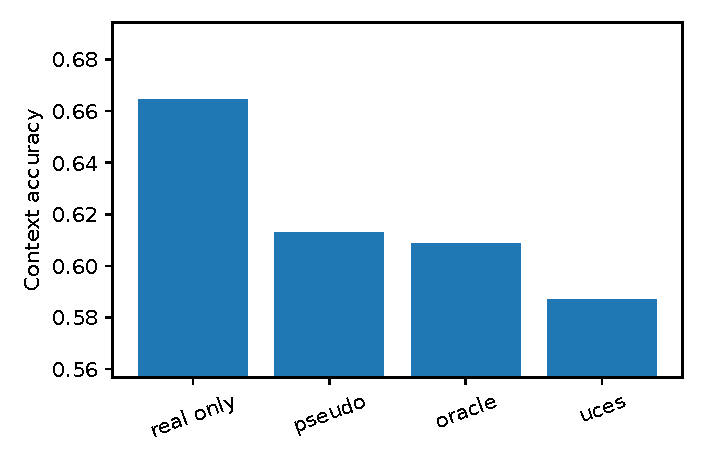
\includegraphics[width=\columnwidth]{../results/paper_figures/oracle_pseudo.pdf}
\caption{Oracle labels do not close the utility gap.}
\end{figure}

\subsection{Evidence mass predicts the degradation}
We next hold the selection rule fixed and sweep both the number of selected synthetic samples $k$ and their per-event reliability weight. Figure~\ref{fig:mass} shows a near-monotonic degradation as synthetic evidence mass $k\times w$ increases. Across non-zero settings, the correlation between synthetic mass and the held-out accuracy delta is $r=-0.988$. At the most conservative setting ($k=1,w=0.08$), the delta is -0.29 percentage points; at $k=8,w=0.50$, it is -7.11 points.

This pattern is consistent with \emph{redundancy amplification}: synthetic samples recapitulate inferred beliefs, so adding them repeatedly changes feature/evidence balance even when each label is correct. In other words, ``correct synthetic data'' is not neutral data.

\begin{figure}[t]
\centering
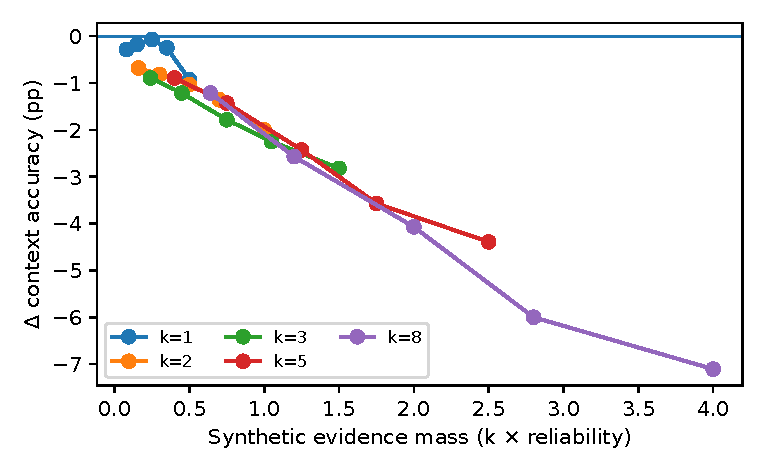
\includegraphics[width=\columnwidth]{../results/paper_figures/synthetic_mass_harm.pdf}
\caption{Synthetic evidence mass strongly predicts downstream harm.}\label{fig:mass}
\end{figure}


\subsection{Dataset-level mass control mitigates the harm}
The mechanism suggests a direct mitigation: control augmentation at the dataset level rather than only scoring individual samples. We cap total synthetic reliability per user at 0.16 and discount repeated $(\text{preference},\text{context})$ signatures. Across five independent seeds (Table~\ref{tab:masscap}), raw utility-calibrated augmentation reduces accuracy by 3.25 percentage points relative to real-only training, whereas mass-capped augmentation reduces it by only 0.18 points. This recovers 94.5\% of the observed degradation. Mass capping improves over raw augmentation in all five seeds, but with only five paired seeds the two-sided exact sign test is still $p=0.0625$. The capped method does \emph{not} provide a statistically established gain over real-only training; its value is as a consistent mitigation that makes the diagnosed mechanism actionable.

\begin{table}[t]
\centering\small
\begin{tabular}{lcc}\toprule
Training evidence & Mean accuracy & $\Delta$ vs. real\\\midrule
Real only & \textbf{0.660} & --\\
Raw utility-calibrated synthetic & 0.627 & -0.032\\
Mass-capped utility synthetic & 0.658 & -0.002\\\bottomrule
\end{tabular}
\caption{Dataset-level mass control neutralizes most augmentation harm across five seeds.}\label{tab:masscap}
\end{table}

\begin{figure}[t]
\centering
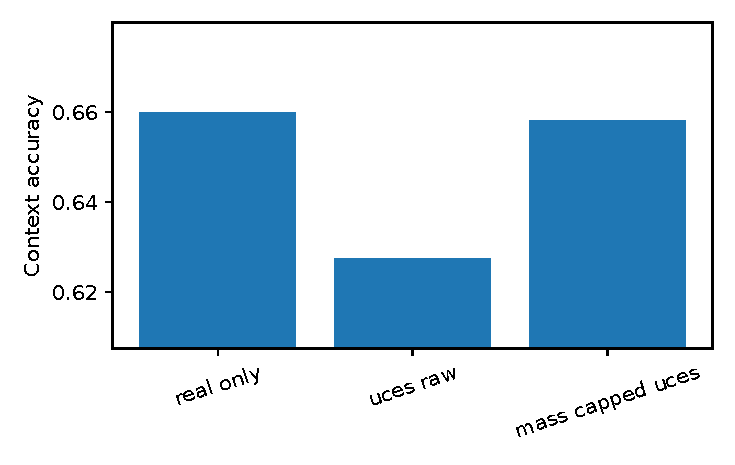
\includegraphics[width=0.95\columnwidth]{../results/paper_figures/mass_control.pdf}
\caption{Mass capping recovers most of the degradation without creating a spurious improvement claim.}\label{fig:masscap}
\end{figure}

\subsection{Selective personalization exposes a risk--coverage tradeoff}
A personal agent should not personalize every query. Figure~\ref{fig:risk} reports risk among cases retained above posterior-confidence thresholds. Moving from near-full coverage toward more selective personalization reduces conditional error before the curve flattens. This supports reporting personalization as a selective decision rather than a binary capability score.

\begin{figure}[t]
\centering
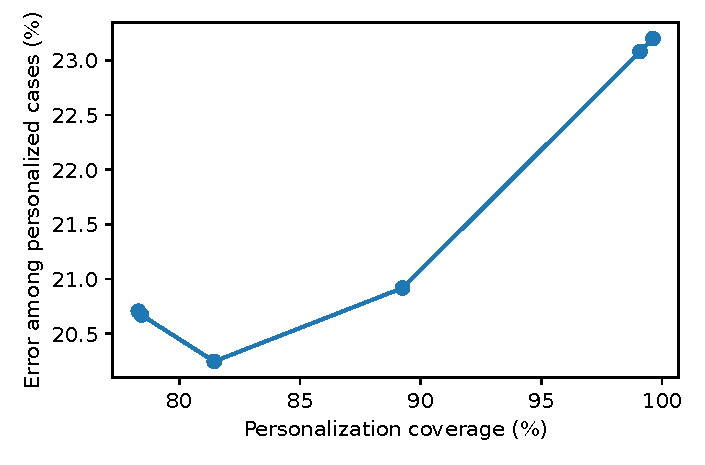
\includegraphics[width=0.95\columnwidth]{../results/paper_figures/risk_coverage.pdf}
\caption{Risk--coverage for context-conditioned personalization.}\label{fig:risk}
\end{figure}


\subsection{State quality transfers to response choice}
Slot accuracy is insufficient if inferred preferences do not change user-facing behavior. We therefore construct natural-language response-selection tasks spanning all preference dimensions plus factual queries where personalization is unnecessary. A shared personalization gate decides whether user state should be consulted; the downstream method then chooses among natural-language candidates. Across five independent seeds, the Bayesian state estimator achieves $0.680\pm0.013$ overall response-choice accuracy ($0.653\pm0.015$ on personalized cases), compared with $0.417\pm0.027$ for a generic policy. An always-personalize state policy reaches $0.591\pm0.009$ overall because it over-personalizes 100\% of irrelevant queries. Bayesian state beats always-personalize in all five seeds; as above, five seed-level replications are directionally consistent but not high-powered (two-sided exact sign test $p=0.0625$). A small PyTorch neural response ranker trained from scratch reaches only $0.450\pm0.022$, underscoring that this benchmark does not substitute for pretrained language-model evaluation.

\begin{figure}[t]
\centering
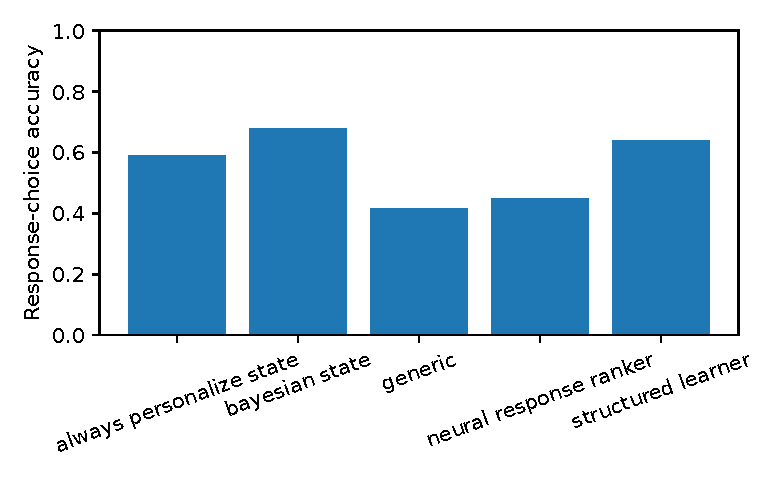
\includegraphics[width=0.95\columnwidth]{../results/paper_figures/response_level.pdf}
\caption{Response-level personalization requires both user-state quality and restraint.}\label{fig:response}
\end{figure}

\subsection{Personalization regret falls with real evidence}
The regret curve (Figure~\ref{fig:regret}) measures decision loss caused by incorrect or missing user-state estimates. Mean regret drops from 0.869 after one real interaction to 0.199 after twenty. Unlike raw slot accuracy, this metric can be replaced by domain utility when evaluating recommendations, actions, or tool use.

\begin{figure}[t]
\centering
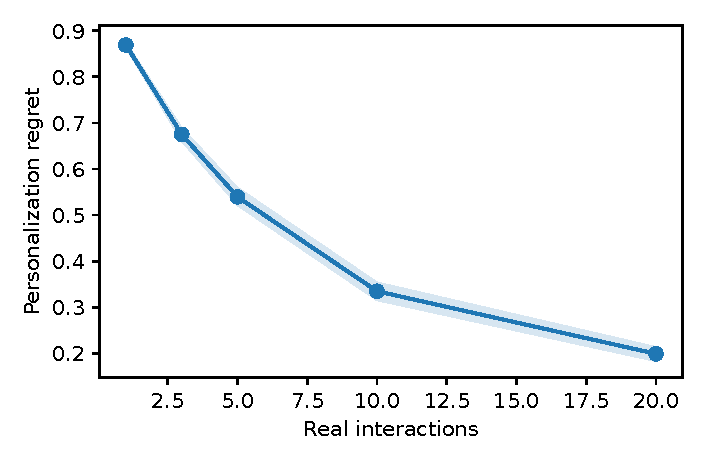
\includegraphics[width=0.95\columnwidth]{../results/paper_figures/regret_curve.pdf}
\caption{Personalization regret versus real interaction count.}\label{fig:regret}
\end{figure}

\subsection{Preference drift should be evaluated against standard detectors}
On a noisy induced-shift benchmark, the original hand-written drift heuristic reaches ROC-AUC 0.928. EWMA and CUSUM baselines reach 0.980 and 0.981, while a posterior-shift score reaches 0.969. The result is intentionally unfavorable to the bespoke heuristic: personalization systems should compare change detectors against standard online baselines instead of treating a custom drift score as evidence of novelty.

\section{Discussion}
\paragraph{Why can oracle-correct synthetic data hurt?}
The experiments separate label correctness from downstream utility. The trainable learner converts a user's interaction history into weighted features. Adding synthetic events therefore does more than provide additional labels: it changes the relative mass assigned to values and contexts. When synthetic examples are generated from an already inferred state, they are correlated with the learner's current belief. Repetition can amplify this belief and reduce sensitivity to held-out real evidence. This is a user-conditioned form of confirmation bias in our controlled setting because the pseudo-data distribution is conditioned on a user model estimated from the same sparse history.

\paragraph{Implication for synthetic-data pipelines.}
Sample-level filters are insufficient. A verifier should estimate at least three quantities separately: label correctness, novelty/information value, and \emph{marginal effect on the training distribution}. The last term can require global constraints such as per-user mass budgets, importance weighting, or influence-function estimates. In our controlled setting, an explicit per-user mass budget recovers 94.5\% of the raw augmentation harm across five seeds but does not create a statistically established gain over real-only training. This distinction matters: a mitigation can be useful without being mislabeled as a new accuracy improvement.

\paragraph{Active querying versus synthetic training.}
Our findings suggest a safer use of counterfactual generation: use synthetic scenarios to identify what to ask the user, rather than automatically treating generated labels as new evidence. PAHF-style clarification provides one path for converting synthetic uncertainty into real feedback~\cite{pahf}. Evaluating this hybrid loop with real interaction cost is an important next step.

\section{External and Human Evaluation Protocols}
The repository includes adapters for PersonaMem-style benchmark rows and PAHF-style scenario files, plus a provider-neutral completion interface. We do not report external benchmark numbers without the corresponding public data and model outputs. PersonaMem-v2 currently provides large-scale implicit-persona evaluation, while PAHF exposes embodied and shopping scenarios with preference evolution~\cite{personamemv2,pahf}. These benchmarks are the appropriate gate for any future state-of-the-art claim.

The human-study package pre-specifies randomized pairwise comparison, scenario stratification, multi-rater annotation, and separate ratings for usefulness, personalization appropriateness, over-personalization, factuality, trust, stale preference, and invented preference. No human-population conclusion is drawn from synthetic users.

\section{Limitations}
The primary experiments use categorical synthetic preferences and small discriminative learners. Ground-truth synthetic states supervise the training-user labels, while held-out users are disjoint and test-time inference does not read simulator-only ground-truth metadata; this supports causal diagnosis inside the simulator but is not a substitute for learning from naturally occurring human feedback. The response-level suite adds a trained PyTorch neural ranker over natural-language histories and candidate responses, but it is deliberately not presented as a post-trained language model. The simulator and evaluator share a closed preference ontology and task-family assumptions, so external validity is limited. The observed mass effect may interact with model class: sequence models or gradient-based post-training may respond differently to duplicated evidence. The risk--coverage and regret metrics are useful abstractions but do not replace product-domain utility. Finally, the benchmark does not establish real-user satisfaction, demographic fairness, or external-benchmark state of the art, and it does not model strategic users, privacy expectations, cultural variation, or irreversible actions.

We attempted to provision a local Hugging Face/PEFT training path in the execution environment, but the required packages and model weights were unavailable without network access. The release therefore ships the integration boundary and experimental protocol without inventing model-training results. External LLM post-training remains a required follow-up, not a hidden claim.

\section{Conclusion}
Personalization is not improved merely by adding examples that look informative. In a controlled moving-user benchmark, synthetic augmentation can reduce held-out accuracy even with nearly perfect or oracle labels, and the degradation scales strongly with synthetic evidence mass. The Synthetic Experience Utility Gap therefore has at least two separable causes: label reliability and distributional reweighting. For personal agents, synthetic experience should be treated as an intervention whose downstream effect must be measured, budgeted, and sometimes rejected. This shifts the research question from \emph{how much synthetic personalization data can we generate?} to \emph{when does synthetic evidence earn the right to update a user's model?}

\section*{Reproducibility Statement}
All internal claims are regenerated from source with fixed seeds, bootstrap scripts, and machine-verifiable result files. The release contains tests, benchmark generators, figures, raw CSV/JSON outputs, a claim verifier, and a SHA-256 manifest. The manuscript intentionally distinguishes reproduced internal results from external-model and human-study protocols that have not been executed.


\appendix
\section{Appendix: Experimental Details}
\subsection{Simulator and ontology}
Each synthetic user contains categorical preferences sampled from a fixed ontology spanning communication style, risk tolerance, planning style, travel priority, autonomy, schedule preference, and related decision attributes. A configurable fraction of attributes receive context-specific overrides. Interaction events carry an event identifier, user identifier, preference key, observed value, signal type, reliability, context, relevance flag, and metadata. The reference experiments treat metadata as non-authoritative so free-form strings cannot overwrite preference values.

The benchmark separates train and held-out users. Context-conditioned labels are evaluated over \{general, work, travel, high-stakes, casual\}. Synthetic candidate generation additionally uses low-stakes, time-pressure, and shared-context probes to expose state estimates to off-distribution contexts; only accepted candidates enter augmentation experiments.

\subsection{Preference posterior}
The categorical posterior uses a symmetric Dirichlet prior with $\alpha=0.65$. Explicit corrections receive a 1.35 multiplicative weight. When evaluating a specific context, evidence from that context receives full weight and other contexts receive a 0.28 backoff weight. These constants are fixed before the paper experiments. We report risk--coverage rather than presenting the posterior probabilities as perfectly calibrated probabilities of user satisfaction.

\subsection{Synthetic experience verifier}
The reference verifier computes plausibility, consistency, novelty, information value, and hallucination risk. It is intentionally simple so the synthetic-utility experiment remains interpretable. A candidate is accepted when a fixed weighted score exceeds the reference threshold. The utility-calibrated selector then estimates a context-conditioned label probability $q(x)$ and subtracts an expected-harm term. Crucially, the oracle-label experiment bypasses pseudo-label correctness entirely; its degradation demonstrates that a better verifier alone cannot guarantee downstream gain.

\subsection{Mass sweep}
We vary the number of selected examples $k\in\{1,2,3,5,8\}$ and event reliability $w\in\{0.08,0.15,0.25,0.35,0.50\}$. We define synthetic evidence mass as $m=k\times w$. The sweep contains 25 non-zero settings plus the real-only reference. No setting in this sweep provides a consistent gain over real-only training. The strongest degradation occurs at $m=4.0$, where accuracy falls by 7.11 percentage points. The sample correlation between mass and the downstream delta is $-0.988$.


\subsection{Mass-capped mitigation}
The mitigation experiment uses five independent seeds. Raw UCES-selected events carry reliability 0.35. The mass-controlled variant caps total synthetic reliability per user at 0.16 and additionally discounts repeated $(\text{preference},\text{context})$ signatures. Mean real-only accuracy is 0.660, raw UCES accuracy is 0.627, and mass-capped UCES accuracy is 0.658. Relative to the 3.25-point raw degradation, the capped variant leaves 0.18 points of degradation, recovering 94.5\% of the harm. We report this as mitigation rather than improvement.

\subsection{Response-level evaluation}
The response suite uses held-out users and natural-language candidate answers for answer detail, planning style, risk tolerance, travel priority, autonomy, privacy sensitivity, and work-time preferences. It also contains factual tasks where all personalized embellishments are irrelevant. The structured baselines share a learned semantic gate; an always-personalize baseline bypasses the gate. The neural response ranker is implemented in PyTorch using a trainable hashed token embedding, explicit history--candidate overlap features, and a small multilayer scoring head. It receives no pretrained language representation. Its weak result is retained as a negative baseline rather than omitted.

\subsection{Selective personalization}
The risk--coverage experiment evaluates 250 held-out users. A prediction is retained only when posterior confidence exceeds threshold $\tau$. Coverage is the fraction of candidate personalization decisions retained; risk is the conditional error among retained decisions. This framing prevents an always-personalize system from appearing strong merely because the benchmark contains many easy preference slots.

\subsection{Drift benchmark}
The drift diagnostic contains 320 balanced changed/stationary cases. Historical evidence includes 12\% observation noise; after a true change, the new value is observed with probability 0.76, while stationary controls contain 18\% spurious alternative observations. The custom heuristic reaches ROC-AUC 0.928, EWMA 0.980, CUSUM 0.981, and posterior total-variation shift 0.969. We include these baselines specifically to avoid presenting a bespoke detector as a research contribution without comparison.

\section{Appendix: External Benchmark Gate}
A state-of-the-art claim is disabled by design until the method is run on recognized external benchmarks with matched contemporary baselines. The release includes parsers for PersonaMem-style question CSV files and PAHF-style JSON scenarios. Third-party data are not redistributed.

For PersonaMem, the intended protocol is: (1) load the official benchmark split; (2) freeze the model and prompt configuration; (3) compare full-history, recent-$K$, retrieval, summarized-profile, structured-state, and benchmark-native baselines; (4) report both multiple-choice and open-ended metrics when supported; and (5) retain raw outputs and benchmark identifiers. For PAHF, the intended protocol compares no-memory, memory, clarification, and correction-enabled configurations across original and evolved-persona phases.

\subsection{Open-weight post-training gate}
The repository includes an SFT JSONL builder and a dependency check for PyTorch, Transformers, PEFT, and Datasets. A valid post-training result must record the base checkpoint, tokenizer revision, training data hash, optimization hyperparameters, adapter/checkpoint hash, random seed, and raw evaluation outputs. During construction of this release, PyTorch was available but Transformers/PEFT/Datasets and model weights were not retrievable because the execution environment had no package/model network access. Consequently, no open-weight or frontier-model result is claimed.

\section{Appendix: Human Evaluation Protocol}
The pre-specified study uses blinded pairwise comparisons between a personalized system and an appropriate baseline. Left/right order is randomized. Scenarios are stratified by cold start, stable preference, context dependence, preference drift, ambiguous evidence, conflicting evidence, and cases where personalization should be withheld. Ratings separate overall task quality from personalization appropriateness, correctness, over-personalization, intrusiveness, factuality, trust, stale-preference use, and invented-preference use.

The analysis reports pairwise win rate with bootstrap confidence intervals, per-scenario breakdowns, rater agreement, and disagreement cases. A future longitudinal study should additionally report correction burden, interactions-to-recovery, and personalization regret under real user utility. Synthetic-user metrics are not substituted for human-population estimates.

\paragraph{Power planning.} A normal-approximation planning calculation (two-sided $\alpha=0.05$, target power 0.80) estimates approximately 194 independent judgments to distinguish a 60\% pairwise win rate from chance, 134 for 62\%, and 85 for 65\%. These are judgment-level approximations rather than participant counts; repeated-measures deployment should inflate for within-participant clustering and report participant-level uncertainty. No recruited-participant result is reported here.

\section{Appendix: Reproducibility and Failure Taxonomy}
The release provides deterministic seeds, raw CSV/JSON result files, figure-building scripts, automated tests, a claim verifier, and a manifest. Failure analysis distinguishes stale-state errors, context leakage, over-personalization, insufficient evidence, conflict resolution failures, synthetic evidence amplification, and grader disagreement. Negative results remain in the repository and are not removed from headline analyses.

A key practical lesson is that per-sample verification and dataset-level control solve different problems. Label calibration addresses whether a candidate is locally trustworthy. Evidence-mass control addresses how many correlated candidates are allowed to alter the effective training distribution. The oracle experiment demonstrates why both levels must be measured.

\begin{thebibliography}{10}\small
\bibitem{personamem} Z. Jiang et al. \emph{Know Me, Respond to Me: Benchmarking LLMs for Dynamic User Profiling and Personalized Responses at Scale}. arXiv:2504.14225.
\bibitem{personamemv2} B. Yu et al. \emph{PersonaMem-v2: Towards Personalized Intelligence via Learning Implicit User Personas and Agentic Memory}. Public benchmark repository.
\bibitem{pahf} K. Liang et al. \emph{Learning Personalized Agents from Human Feedback}. arXiv:2602.16173.
\bibitem{prefpalette} J. Li et al. \emph{PrefPalette: Personalized Preference Modeling with Counterfactual Attribute Synthesis}. arXiv:2507.13541.
\bibitem{beyond} Y. Zhang et al. \emph{Beyond Similarity: Trustworthy Memory Search for Personal AI Agents}. arXiv:2606.06054.
\bibitem{lamp} A. Salemi, S. Mysore, M. Bendersky, and H. Zamani. \emph{LaMP: When Large Language Models Meet Personalization}. ACL, 2024.
\bibitem{memorybank} W. Zhong, L. Guo, Q. Gao, H. Ye, and Y. Wang. \emph{MemoryBank: Enhancing Large Language Models with Long-Term Memory}. AAAI, 2024.
\bibitem{memgpt} C. Packer, S. Wooders, K. Lin, V. Fang, S. G. Patil, I. Stoica, and J. E. Gonzalez. \emph{MemGPT: Towards LLMs as Operating Systems}. arXiv:2310.08560.
\bibitem{mem0} P. Chhikara, D. Khant, S. Aryan, T. Singh, and D. Yadav. \emph{Mem0: Building Production-Ready AI Agents with Scalable Long-Term Memory}. arXiv:2504.19413.
\bibitem{amem} W. Xu, Z. Liang, K. Mei, H. Gao, J. Tan, and Y. Zhang. \emph{A-MEM: Agentic Memory for LLM Agents}. NeurIPS, 2025.
\bibitem{spring} S. Kim and J. Kim. \emph{SPRInG: Continual LLM Personalization via Selective Parametric Adaptation and Retrieval-Interpolated Generation}. arXiv:2601.09974.
\bibitem{hypreflect} E. Hwang et al. \emph{Hypotheses-Guided Self Distillation for Continual Personalization}. arXiv:2609.00251.
\bibitem{hypertrace} J. Shen et al. \emph{HyperTrace: Hypothesis-Based Preference Tracing for Online LLM Personalization}. arXiv:2609.09835.
\bibitem{core} Y. Zhang et al. \emph{Toward Robust Personalized Alignment for LLMs: Mitigating Persona Drift in Multi-Turn Dialogue}. arXiv:2609.12373.
\bibitem{cope} R. Cao et al. \emph{COPE: Continual Personalization of LLMs under Sparse User Feedback via User Embeddings and Self-Evaluation}. arXiv:2609.26853.
\bibitem{syntheticusersfail} Z. Chen, D. Zhu, and L. N. Zheng. \emph{When Synthetic Users Fail: A Cross-Domain Benchmark of LLM-Simulated Human Survey Responses}. arXiv:2607.26348.
\bibitem{settles} B. Settles. \emph{Active Learning Literature Survey}. University of Wisconsin--Madison, 2009.
\bibitem{arazo} E. Arazo et al. \emph{Pseudo-Labeling and Confirmation Bias in Deep Semi-Supervised Learning}. IJCNN, 2020.
\bibitem{adams} R. Adams and D. MacKay. \emph{Bayesian Online Changepoint Detection}. arXiv:0710.3742.
\end{thebibliography}
\end{document}
